\documentclass[11pt, aspectratio=169, xcolor=table]{beamer}

% --- Langue et Police ---
\usepackage[utf8]{inputenc}
\usepackage[french]{babel}
\usepackage[T1]{fontenc}
\usepackage{helvet}
\usepackage{tikz}
\usepackage{graphicx}
\usepackage{booktabs}
\usepackage{amsmath}

% --- Interface et Couleurs ---
\usetheme{default}
\usecolortheme{whale}

\definecolor{MainNavy}{RGB}{0, 51, 102}
\definecolor{MainGold}{RGB}{184, 152, 75}
\definecolor{SubGray}{RGB}{128, 128, 128}

\setbeamercolor{title}{fg=MainNavy}
\setbeamercolor{subtitle}{fg=SubGray}
\setbeamercolor{author}{fg=black}
\setbeamercolor{institute}{fg=black}
\setbeamercolor{frametitle}{bg=MainNavy, fg=white}

% --- Retirer les éléments superflus ---
\setbeamertemplate{navigation symbols}{}

% --- Personnalisation de la page de titre ---
\setbeamertemplate{title page}{
    \begin{center}
        \begin{figure}[H]
            \centering
            \begin{minipage}{0.3\textwidth}
                \centering
                
\includegraphics[width=0.8\textwidth]{figures/logo-INSA.png}
            \end{minipage}
            \hfill
            \begin{minipage}{0.3\textwidth}
                \centering
                
\includegraphics[width=0.5\textwidth]{figures/logo-torus.png} 
            \end{minipage}
            \hfill
            \begin{minipage}{0.3\textwidth}
                \centering
                
\includegraphics[width=0.8\textwidth]{figures/logo-N7.png}
            \end{minipage}
        \end{figure}
        
        \vspace{0.5cm}
        
        {\large\color{SubGray} \insertsubtitle}
        \vspace{0.4cm}

        {\Large\bfseries\color{MainNavy} \inserttitle}

        \vfill
        
        \begin{columns}[t]
            \hfill
            \begin{column}{0.5\textwidth}
                \small
                \textbf{Auteur :} Minh Duy Nguyen \\
                \textbf{Filière :} Modélisation Mathématique \& IA \\
                \textbf{Maître de stage :} Milad Mozafari (Torus AI) \\
                \textbf{Date de soutenance :} 05/02/2026
            \end{column}
            
            \vrule{} 
            \hfill
            
            \begin{column}{0.3\textwidth}
               \small
                \textbf{Jury} \\
                David Bertoin \\
                Charles Dossal \\
                Olivier Roustant
            \end{column}
            \hfill
        \end{columns}
    \end{center}
}

% --- Informations du document ---
\title{Optimisation et Adaptation des Modèles de Langage pour des Tâches Spécifiques au Domaine}
\subtitle{Rapport de Stage de Fin d'Études}
\author{Minh Duy Nguyen}
\institute{Milad Mozafari (Torus AI) \& David Bertoin (INSA Toulouse)}
\date{}

\begin{document}

% Slide de titre
\begin{frame}[plain]
    \titlepage
\end{frame}

\begin{frame}{Plan de la Présentation}
    \tableofcontents
\end{frame}

\section{Introduction}

\begin{frame}{De la Recherche à la Pratique : Défis de l'Implémentation de l'IA en Entreprise}
    \textbf{Constat :} 95\% des projets d'IA générative/LLM en entreprise échouent à générer une valeur significative.\\
    \vspace{0.3cm}
    
    \textbf{Deux Défis Fondamentaux en NLP Spécifique au Domaine :}
    \vspace{0.2cm}
    
    \begin{columns}[T]
        \column{0.48\textwidth}
        \begin{alertblock}{Lacune de Connaissances}
            \begin{itemize}
                \item Données d'entraînement statiques
                \item Risques d'hallucinations
                \item Pas d'accès aux documents propriétaires
            \end{itemize}
        \end{alertblock}

        \column{0.48\textwidth}
        \begin{alertblock}{Lacune Comportementale}
            \begin{itemize}
                \item Incapacité à suivre les workflows du domaine
                \item Dérive hors caractère
            \end{itemize}
        \end{alertblock}
    \end{columns}

    \vspace{0.3cm}
    \begin{center}
        \textbf{\color{MainNavy} Comment combler ces lacunes avec un déploiement à ressources limitées ?}
    \end{center}
\end{frame}

% ========== NOUVELLE SLIDE DE TRANSITION ==========
\begin{frame}{Combler les Lacunes : Deux Approches Complémentaires}
    \begin{columns}[T]
        \column{0.48\textwidth}
        \begin{block}{Traiter la Lacune de Connaissances}
            \textbf{Approches Courantes :}
            \begin{itemize}
                \item Pré-entraînement continu
                \item Ingénierie de prompts
                \item \textbf{\color{MainNavy}Génération Augmentée par Récupération (RAG)}
                \item Intégration d'API
            \end{itemize} 
        \end{block}

        \column{0.48\textwidth}
        \begin{block}{Traiter la Lacune Comportementale}
            \textbf{Approches Courantes :}
            \begin{itemize}
                \item Ingénierie de prompts complexe
                \item Apprentissage few-shot
                \item \textbf{\color{MainNavy}Fine-tuning}
                \item RLHF
            \end{itemize}  
        \end{block}
    \end{columns}
    
    \vspace{0.4cm}
    \begin{center}
        \textbf{\color{MainNavy}Ce travail explore les deux approches avec des applications réelles}
    \end{center}
\end{frame}

% ========== SECTION 2 : PROBLÈME 1 ==========
\section{Problème 1 : Intégration de Connaissances Externes pour les Modèles de Langage}

% Slide de séparation de section
\begin{frame}[plain]
    \begin{center}
        \vfill
        {\Huge\color{MainNavy}\textbf{Problème 1}}
        \vspace{0.5cm}
        
        {\Large Intégration de Connaissances Externes pour les Modèles de Langage}
        \vspace{0.3cm}
        
        {\large Construction d'un Système RAG pour Documents Complexes}
        \vfill
    \end{center}
\end{frame}

\begin{frame}{Problème 1 : Intégration de Connaissances Externes}
    \begin{block}{Cas d'usage : Construction d'un système de QA spécifique au domaine pour documents financiers et médicaux}
        \begin{itemize}
            \item \textbf{Objectif :} Permettre des réponses précises aux questions sur des documents complexes et propriétaires
            \item \textbf{Contraintes :} Haute précision, faible latence, déploiement économique
        \end{itemize}
    \end{block}
    
    \vspace{0.3cm}
    \textbf{Questions Clés :}
    \begin{itemize}
        \item Comment préserver la structure dans les documents complexes ?
        \item Comment garantir une haute précision avec des ressources limitées ?
        \item Comment traiter efficacement les données multimodales ?
    \end{itemize}
\end{frame}

\begin{frame}{Le Vrai Défi : Données Financières Complexes}
    \begin{columns}[t]
        \begin{column}{0.48\textwidth}
            \textbf{\color{MainNavy} Cas d'Étude 1 : Finance - Rapports GPM}
            \vspace{0.2cm}
            
            \small Tableaux et graphiques financiers complexes
            
            \vspace{0.4cm}
            \centering
            \fbox{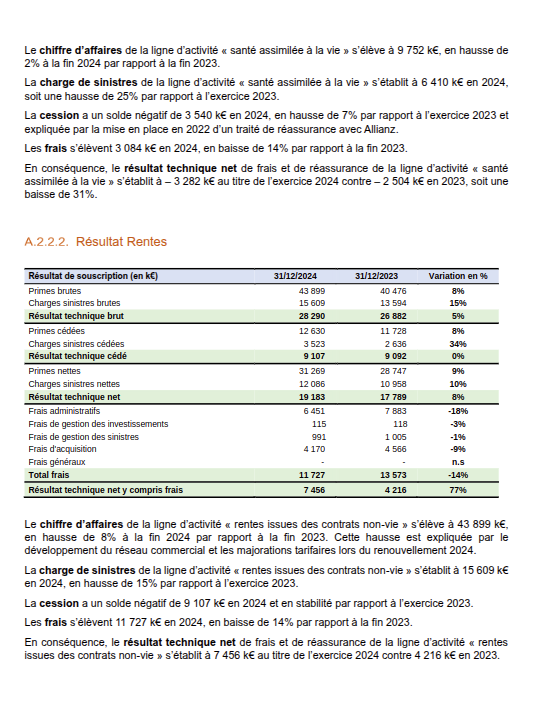
\includegraphics[width=\textwidth]{figures/gpm_report_example.png}} 
        \end{column}

        \begin{column}{0.48\textwidth}
            \textbf{Objectif}
            \begin{itemize}
                \item Recherche rapide d'informations dans les rapports financiers annuels
            \end{itemize}

            \textbf{Défis}
            \begin{itemize}
                \item Données multi-modales : bilans, tableaux, graphiques, images
                \item Documents longs (50-200 pages)
                \item Préservation des relations entre les points de données
            \end{itemize}
        \end{column}
    \end{columns}
\end{frame}

\begin{frame}{Le Vrai Défi : Données Médicales Complexes}
    \begin{columns}[t]
        \begin{column}{0.48\textwidth}
            \textbf{\color{MainNavy} Cas d'Étude 2 : Santé - Catalogue CCAM}
            \vspace{0.2cm}
            
            \small Des milliers de codes médicaux nécessitant une correspondance exacte
            
            \vspace{0.4cm}
            \centering
            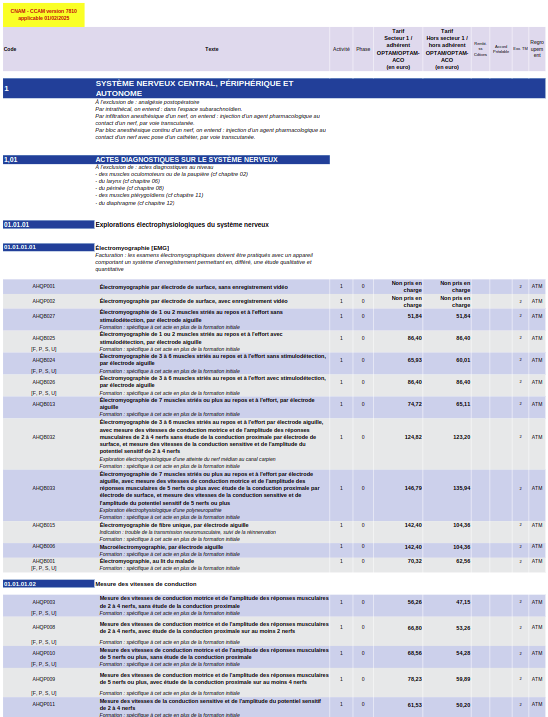
\includegraphics[width=\textwidth]{figures/ccam_example.png}
        \end{column}

        \begin{column}{0.48\textwidth}
            \textbf{Objectif}
            \begin{itemize}
                \item Trouver le(s) bon(s) code(s) médical/médicaux pour des scénarios cliniques donnés
            \end{itemize}

            \textbf{Défis}
            \begin{itemize}
                \item Des milliers de codes dans une structure tabulaire complexe
                \item Correspondance exacte de code requise
                \item Descriptions de codes similaires causant de la confusion
            \end{itemize}
        \end{column}
    \end{columns}
\end{frame}

\begin{frame}{Autres Barrières Techniques}
    \begin{itemize}
        \item \textbf{Contraintes strictes de sécurité des données :} Les données sensibles et privées ne peuvent pas être exposées à ChatGPT ou aux services cloud
        \item \textbf{Exigences de haute précision :} L'hallucination est inacceptable dans les domaines à enjeux élevés comme la finance et la santé
        \item \textbf{Déploiement à ressources limitées :} Les grands modèles nécessitent des ressources computationnelles importantes, tandis que les petits modèles ont des fenêtres de contexte limitées
    \end{itemize}
    
    \vspace{0.5cm}
    \textbf{\color{MainNavy} $\rightarrow$ Objectif de la Solution :} Un pipeline RAG interne unifié capable de gérer des documents complexes avec une haute précision
\end{frame}

\begin{frame}{Pipeline RAG Simple - Approche de Référence}
    \begin{columns}[c]
        \begin{column}{0.48\textwidth}
            \centering
            \includegraphics[width=\textwidth, keepaspectratio]{figures/basic_rag_pipeline.png}
        \end{column}

        \begin{column}{0.48\textwidth}
            \textbf{\color{MainNavy} Configuration RAG Simple}
            \begin{itemize}
                \item \textbf{Analyse :} PyPDF pour l'extraction de texte
                \item \textbf{Découpage :} Taille fixe (512 tokens/chunk, 50 de chevauchement)
                \item \textbf{Embedding :} all-MiniLM-L6-v2 
                \item \textbf{Base Vectorielle :} ChromaDB avec recherche dense
                \item \textbf{Génération :} Gemma-3-12b-it
            \end{itemize}
        \end{column}
    \end{columns}
\end{frame}

\begin{frame}[fragile]{Pourquoi le RAG Simple Échoue : Problème 1 - Perte de Structure de Table}
    \centering
    \textbf{\color{MainNavy}Problème : Aplatissement de la Structure de Table 2D}
    \vspace{0.3cm}
    
    \begin{columns}[c]
        \begin{column}{0.45\textwidth}
            \centering
            \small\textbf{Table Originale :}
            \resizebox{\linewidth}{!}{
            \begin{tabular}{|l|r|r|r|}
                \hline
                \textbf{Sous modules (en k€)} & \textbf{SCR 2024} & \textbf{SCR 2023} & \textbf{Évol.} \\
                \hline
                Type 1 & 2 692 & 2 487 & 8 \% \\
                \hline
                Type 2 & 28 377 & 36 221 & -22 \% \\
                \hline
                Diversification & -621 & -586 & 6 \% \\
                \hline
                \textbf{Risque de défaut} & \textbf{30 448} & \textbf{38 121} & \textbf{-20 \%} \\
                \hline
            \end{tabular}
        }
        \end{column}
        
        \begin{column}{0.05\textwidth}
            \centering $\rightarrow$
        \end{column}
        
        \begin{column}{0.48\textwidth}
            \small\textbf{Sortie PyPDF :}
            \begin{minipage}[t]{0.95\textwidth}
        \tiny
        \begin{verbatim}
Sous modules (en k€) SCR 2024 SCR 2023 Evolution 
Type 1 2 692 2 487 8 % 
Type 2 28 377 36 221 -22 % 
Effet de diversification -621 -586 6 % 
Risque de défaut 30 448 38 121 -20 %
        \end{verbatim}
    \end{minipage}
        \end{column}
    \end{columns}
    
    \vspace{0.3cm}
    \small\textbf{Impact :} Le contexte ligne/colonne est perdu, rendant difficile la compréhension des relations par les LLM
\end{frame}

\begin{frame}{Pourquoi le RAG Simple Échoue : Problème 2 - Échec avec la Correspondance Exacte de Code}
    \textbf{\color{MainNavy}Problème : L'embedding dense a du mal avec la correspondance exacte de mots-clés}
    \vspace{0.3cm}
    
    \begin{columns}[c]
        \begin{column}{0.45\textwidth}
            \centering
            \textbf{Requête Utilisateur :}
            
\includegraphics[width=\textwidth]{figures/search_HAFA.png}
        \end{column}
        
        \begin{column}{0.05\textwidth}
            \centering $\rightarrow$
        \end{column}
        
        \begin{column}{0.48\textwidth}
            \textbf{Résultats de Recherche :}
            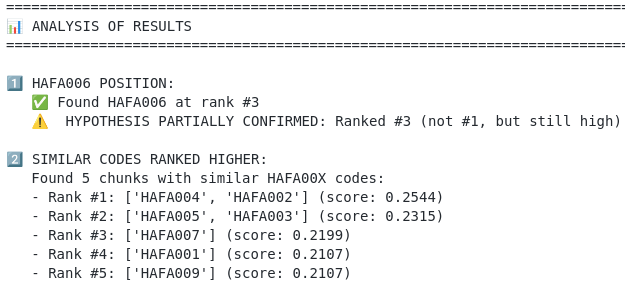
\includegraphics[width=\textwidth]{figures/ccam_dense_search_failure.png}
        \end{column}
    \end{columns}
    
    \vspace{0.3cm}
    \small\textbf{Impact :} Le code exact "HAFA006" n'est pas trouvé dans les premiers résultats ; des codes sémantiquement similaires mais incorrects sont classés plus haut
\end{frame}

\begin{frame}{Pourquoi le RAG Simple Échoue : Analyse Quantitative}
    \textbf{Autres Problèmes :}
    \begin{itemize}
        \item \textbf{Perdu au milieu :} La précision du LLM diminue lorsque le passage de vérité terrain n'est pas en position élevée dans les top-k résultats
        \item \textbf{Incompatibilité d'embedding multilingue :} Modèle d'embedding anglais appliqué aux documents français
    \end{itemize}
    
    \vspace{0.4cm}
    \textbf{\color{MainNavy}Résultats Quantitatifs sur l'Ensemble de Test GPM}
    \begin{table}
        \centering
        \begin{tabular}{|l|c|p{5cm}|}
            \hline
            \textbf{Métrique} & \textbf{Score} & \textbf{Interprétation} \\
            \hline
            Exactitude & 0.66 & Seulement 66\% des réponses correctes par rapport aux contextes \\
            \hline
            Pertinence & 0.73 & 73\% des réponses pertinentes à la question \\
            \hline
        \end{tabular}
    \end{table}
    
    \vspace{0.2cm}
    \textbf{Conclusion :} Le RAG simple n'atteint que 66\% d'exactitude — insuffisant pour les domaines à enjeux élevés
\end{frame}

\begin{frame}{Pipeline RAG Multimodal Avancé - Vue d'Ensemble}
    \begin{columns}[c]
        \begin{column}{0.4\textwidth}
            \textbf{\color{MainNavy}Innovations Clés :}
            \vspace{0.3cm}
            \begin{itemize}
                \item Traitement de documents préservant la structure
                \item Résumé multimodal
                \item Recherche hybride combinant sémantique et mots-clés
                \item Reclassement par cross-encoder
            \end{itemize}
        \end{column}

        \begin{column}{0.6\textwidth}
            \begin{figure}
                \centering
                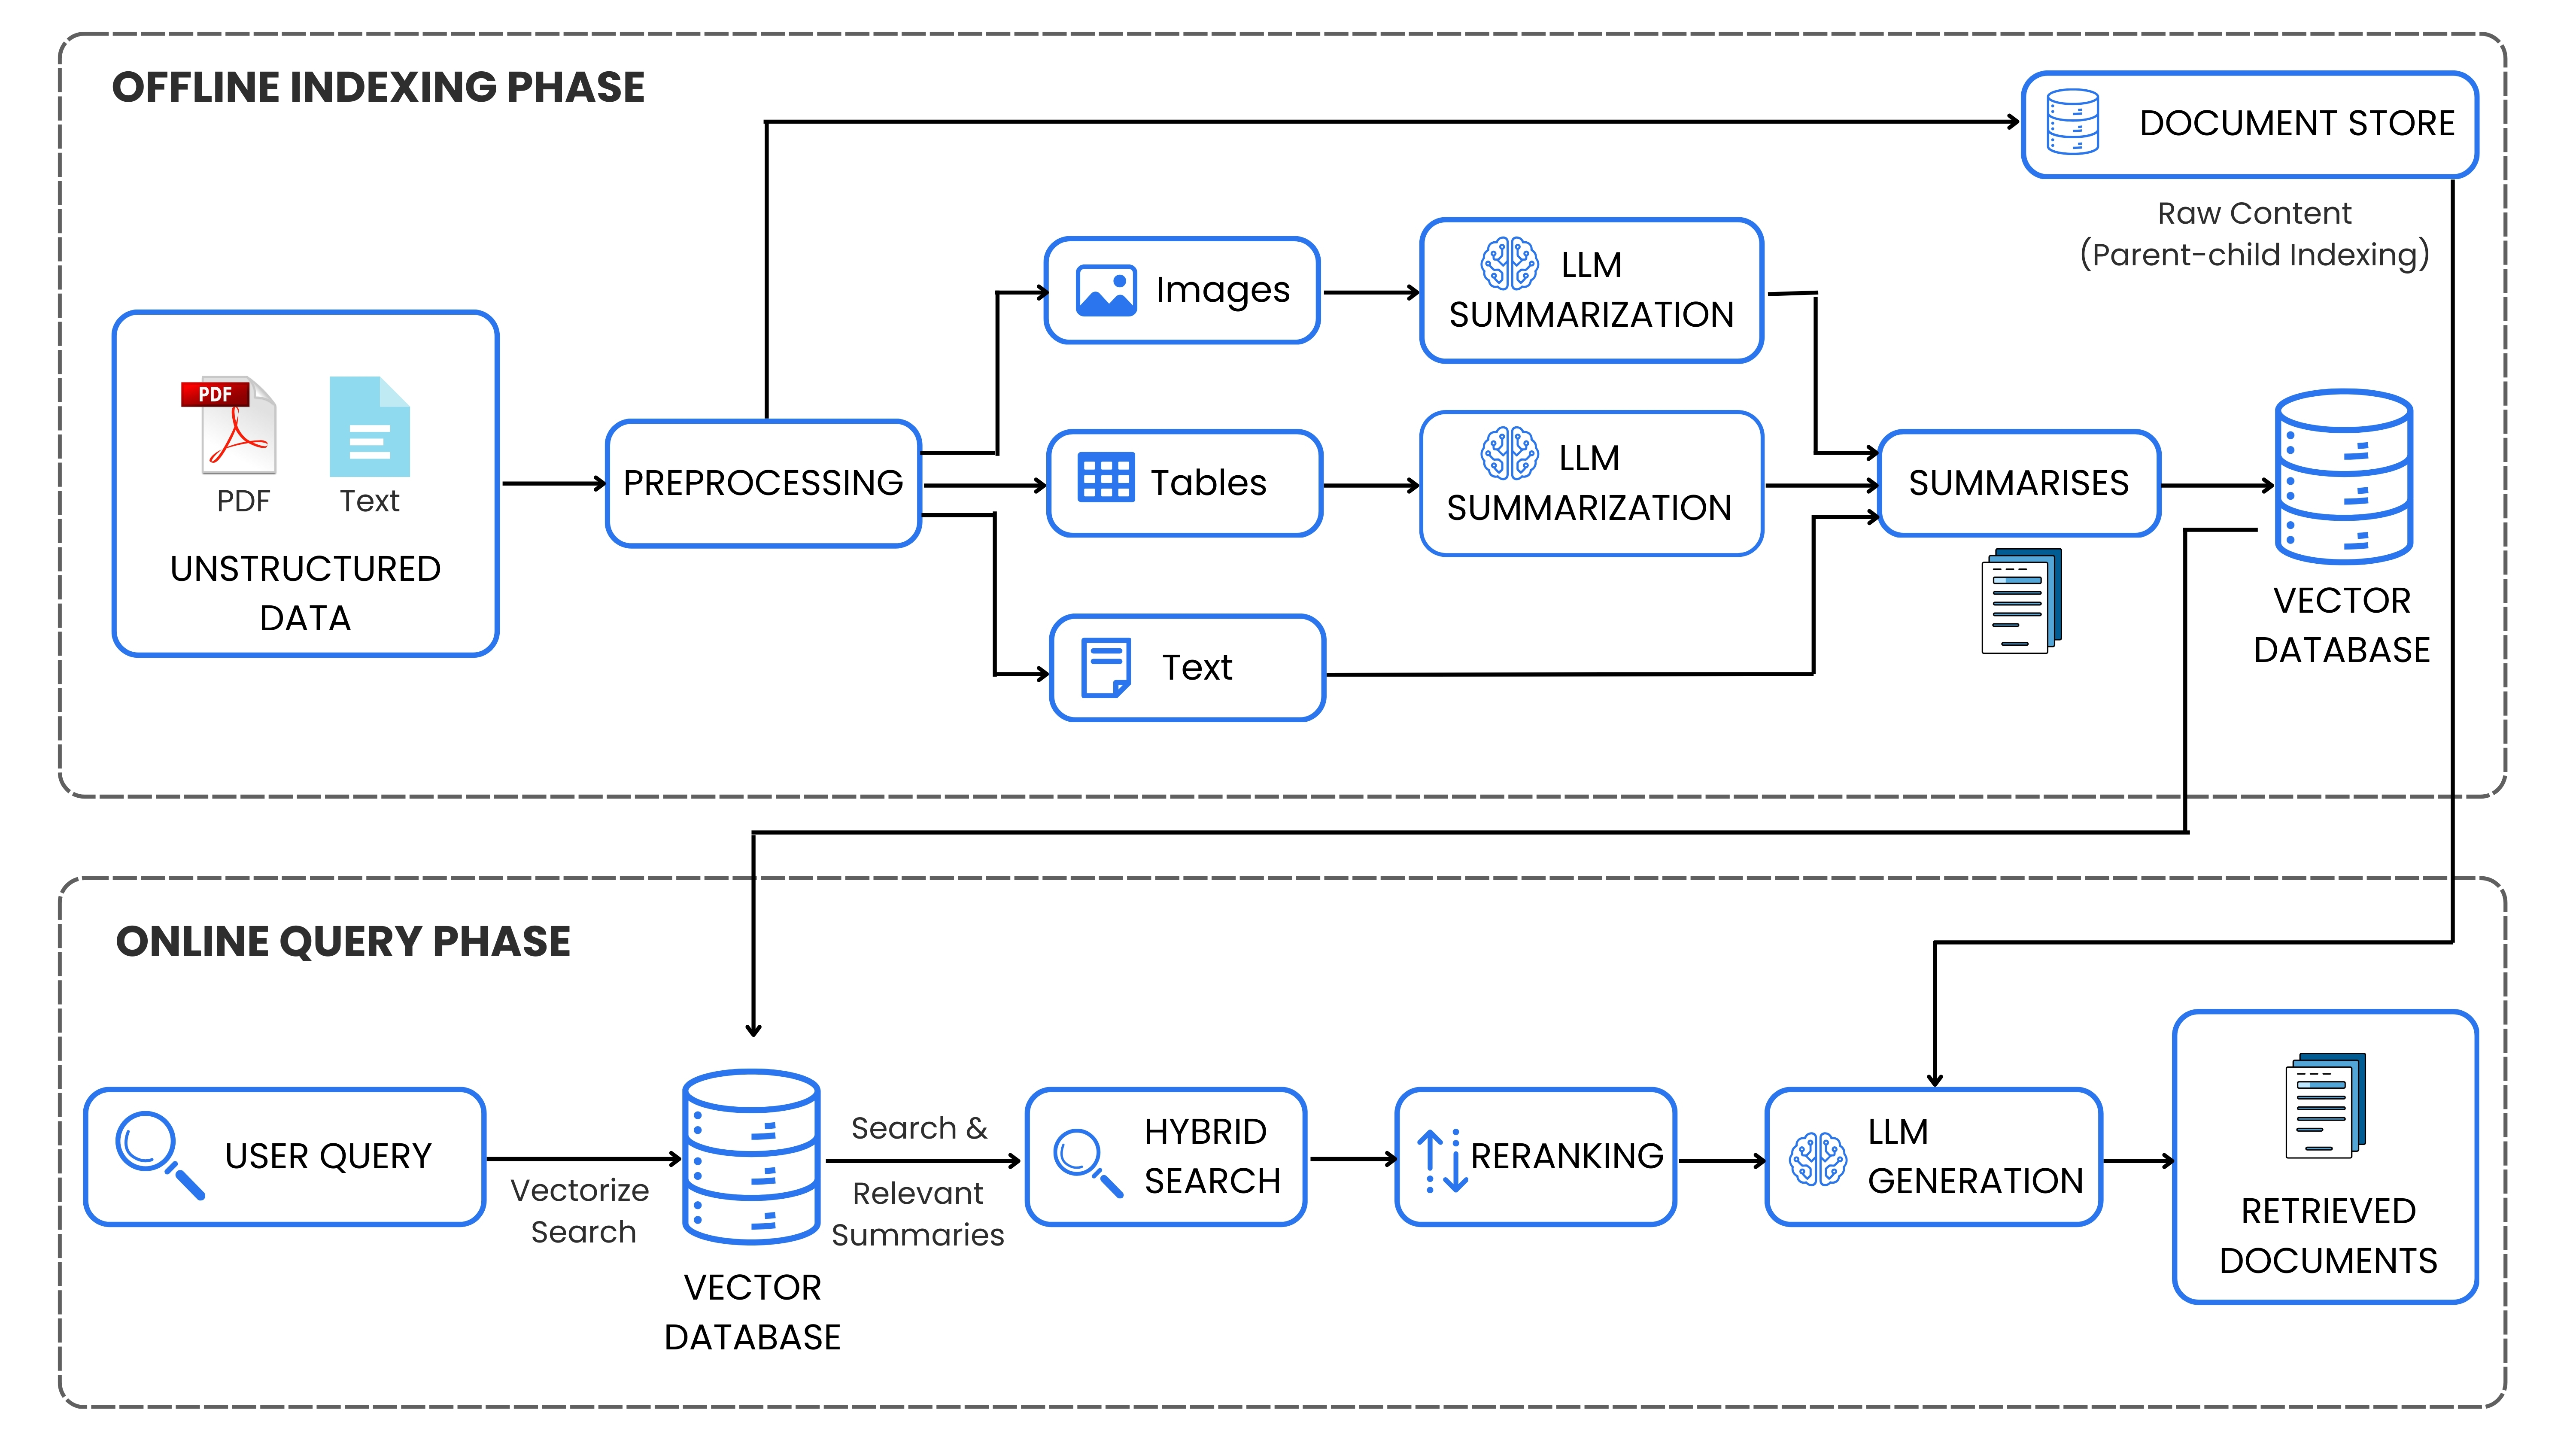
\includegraphics[width=\textwidth]{figures/advanced_rag_pipeline.jpg}
            \end{figure}
        \end{column}
    \end{columns}
\end{frame}

\begin{frame}{Indexation Hors Ligne : Préservation de la Structure}
    \begin{figure}
        \centering
        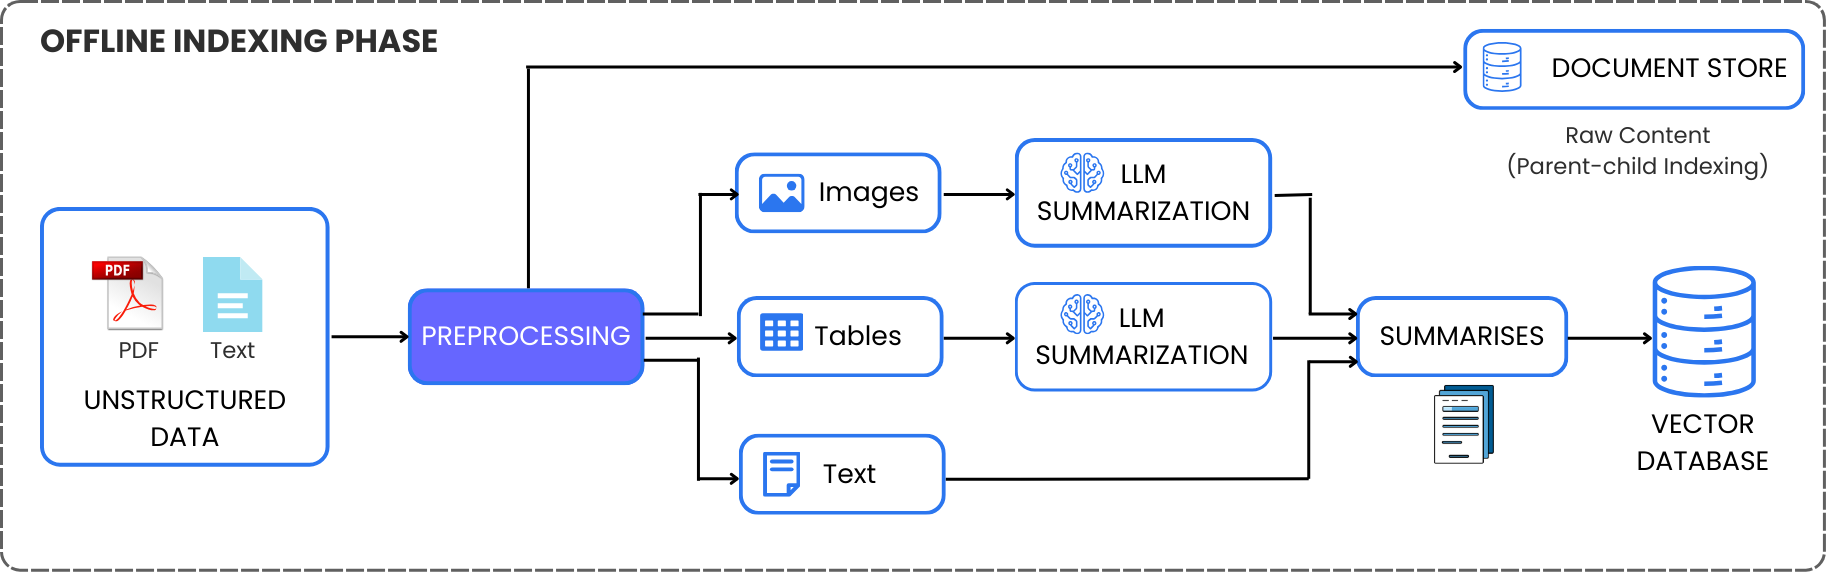
\includegraphics[width=0.75\textwidth]{figures/processing.png}
    \end{figure}
    
    \textbf{Préservation de la Structure avec UnstructuredIO et Table Transformer :}
    \begin{enumerate}
        \item \textbf{Détection de Table :} Identifier les positions des tables en utilisant YoloX/Detectron2
        \item \textbf{Reconnaissance de Structure :} Reconnaître les cellules, cellules fusionnées, en-têtes vs. corps
        \item \textbf{Mapping HTML :} Convertir en balises \texttt{<table>} pour un traitement LLM facile
    \end{enumerate}
\end{frame}

\begin{frame}{Indexation Hors Ligne : Exemple de Préservation de Structure}
    \begin{columns}[c]
        \begin{column}{0.58\textwidth}
            \centering
            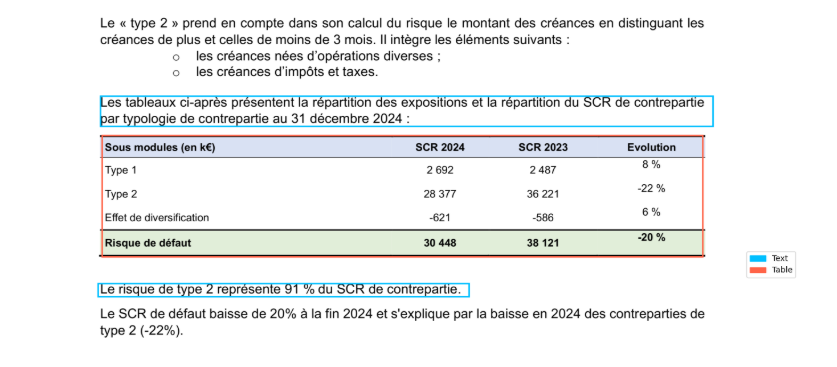
\includegraphics[width=\textwidth, keepaspectratio]{figures/unstructuredio_table_detection.png}
            
            \small L'extraction de table préserve les relations spatiales
        \end{column}
        \begin{column}{0.38\textwidth}
            \centering
            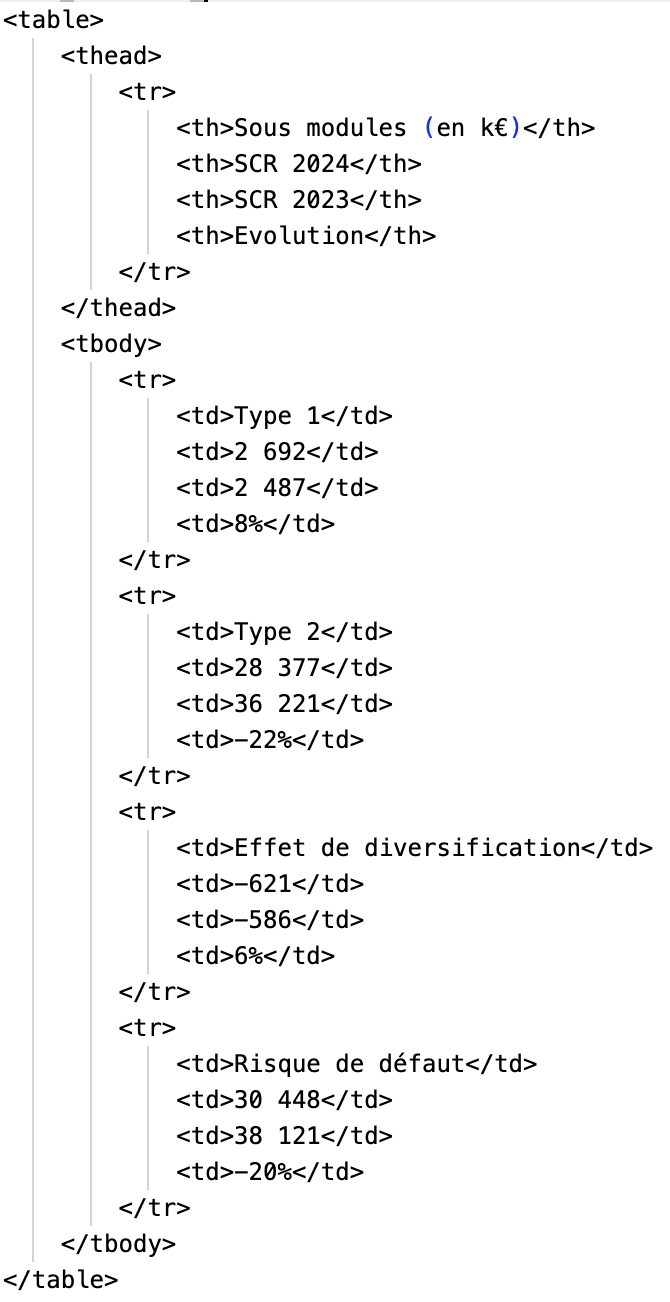
\includegraphics[height=0.8\textheight, keepaspectratio]{figures/html_output.png}
            
            {\small Sortie HTML avec structure intacte}
        \end{column}
    \end{columns}
\end{frame}

\begin{frame}{Indexation Hors Ligne : Résumé Multimodal}
    \begin{figure}
        \centering
        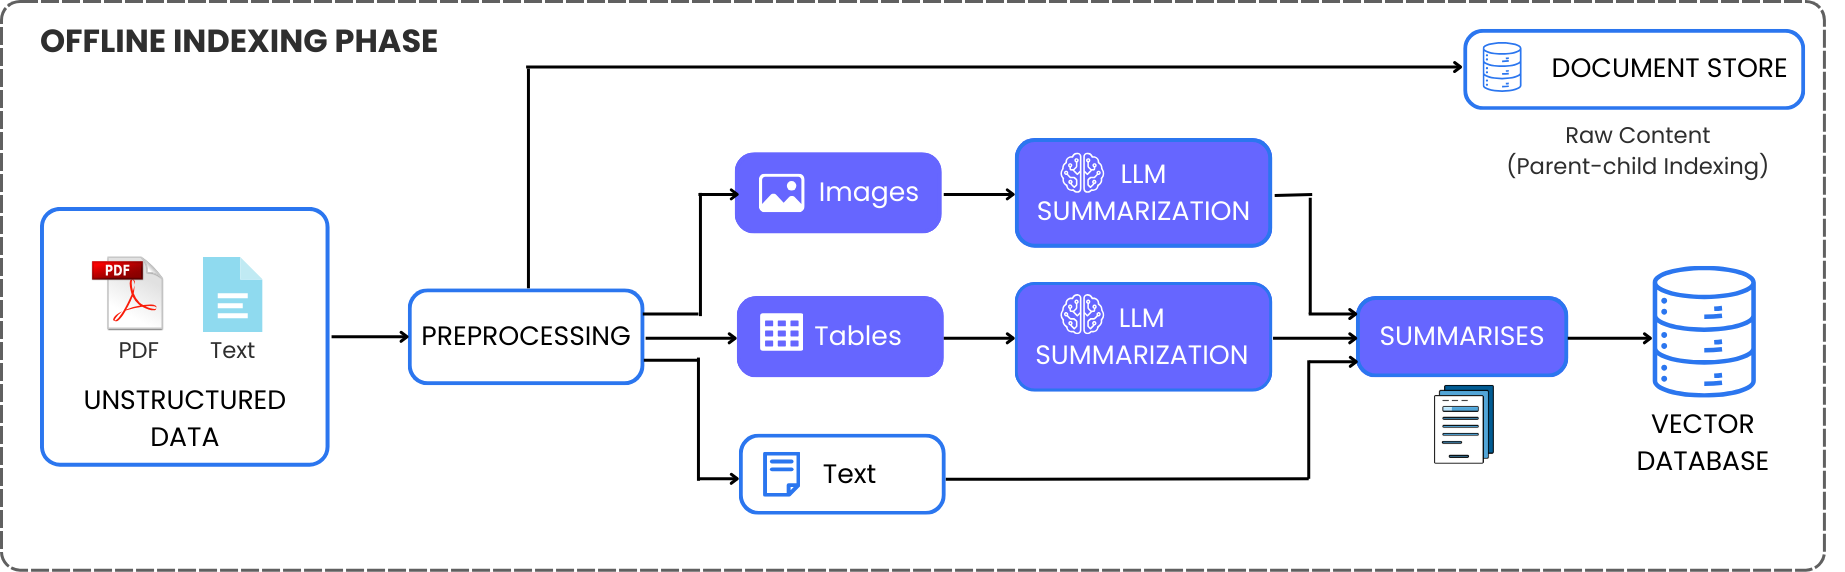
\includegraphics[width=0.7\textwidth]{figures/summarization.png}
    \end{figure}
    
    \textbf{Objectif :} Réduire la taille du contexte tout en préservant les informations clés
    \vspace{0.2cm}
    
    \begin{columns}[c]
        \begin{column}{0.44\textwidth}
            \centering
            \small\textbf{Table Originale :}
            \resizebox{\linewidth}{!}{
            \begin{tabular}{|l|r|r|r|}
                \hline
                \textbf{Sous modules} & \textbf{2024} & \textbf{2023} & \textbf{Évol.} \\
                \hline
                Type 1 & 2 692 & 2 487 & 8 \% \\
                Type 2 & 28 377 & 36 221 & -22 \% \\
                Diversif. & -621 & -586 & 6 \% \\
                \textbf{Total} & \textbf{30 448} & \textbf{38 121} & \textbf{-20 \%} \\
                \hline
            \end{tabular}
        }
        \end{column}
        
        \begin{column}{0.05\textwidth}
            $\rightarrow$
        \end{column}
        
        \begin{column}{0.48\textwidth}
            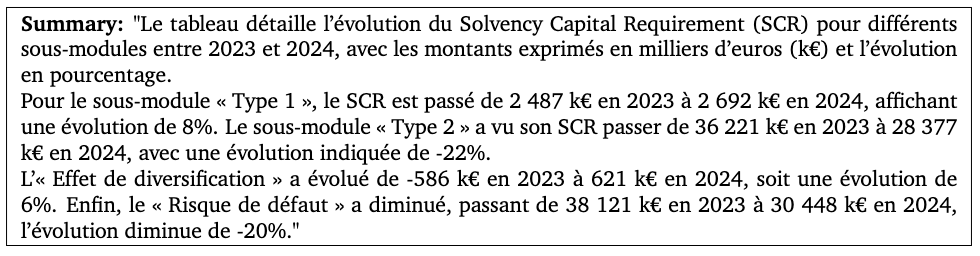
\includegraphics[width=\textwidth, keepaspectratio]{figures/table_summary.png}
        \end{column}
    \end{columns}
\end{frame}

\begin{frame}{Indexation Hors Ligne : Architecture Parent-Enfant}
    \begin{figure}
        \centering
        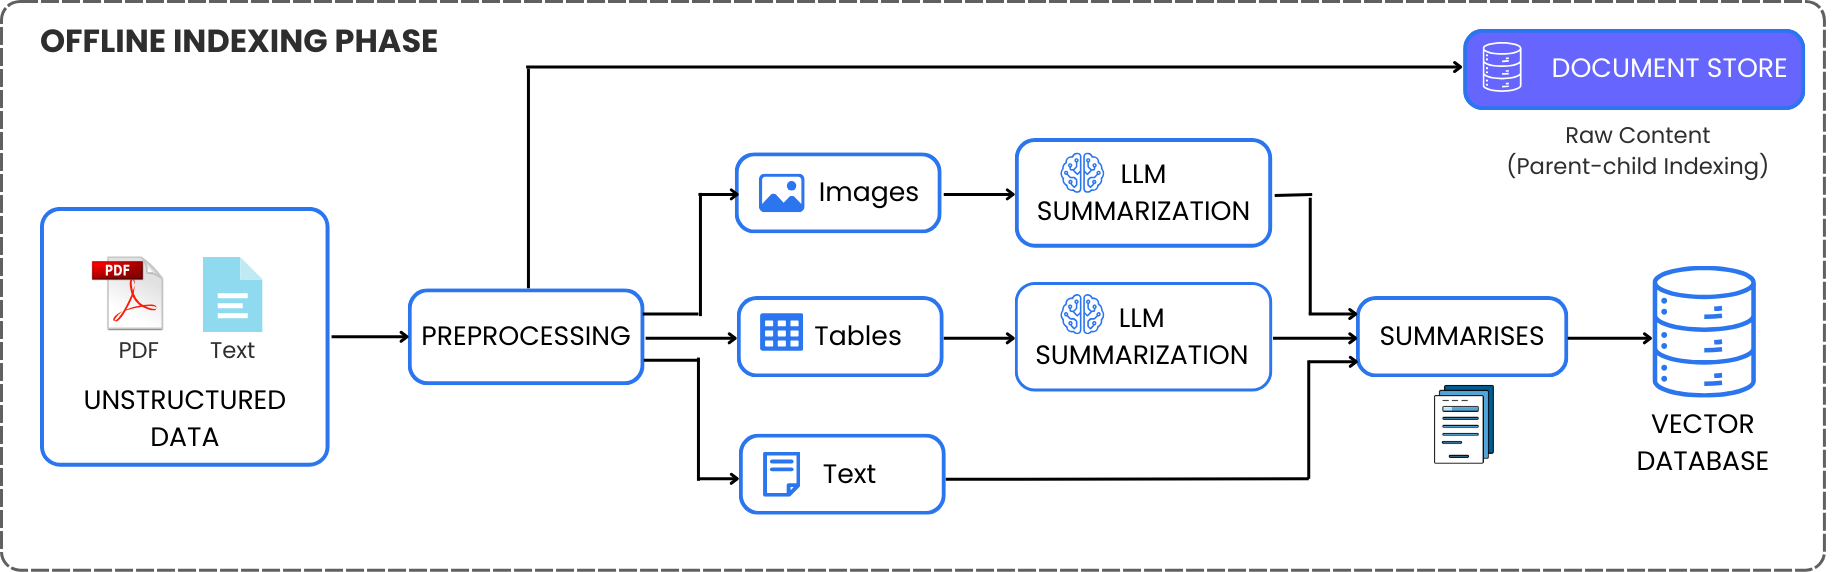
\includegraphics[width=0.58\textwidth, keepaspectratio]{figures/parentchild.png}
    \end{figure}
    
    \textbf{Principe de Conception :}
    \begin{itemize}
        \item \textbf{Enfant (Résumé) :} Stocké dans la base vectorielle pour une récupération efficace
        \item \textbf{Parent (Contenu Brut) :} Stocké dans la base de documents pour une génération détaillée
    \end{itemize}
    
    \vspace{0.2cm}
    \textbf{Avantage :} Récupérer en utilisant des résumés concis, générer en utilisant des informations complètes
\end{frame}

\begin{frame}{Indexation Hors Ligne : Modèle d'Embedding Multilingue}
    \begin{figure}
        \centering
        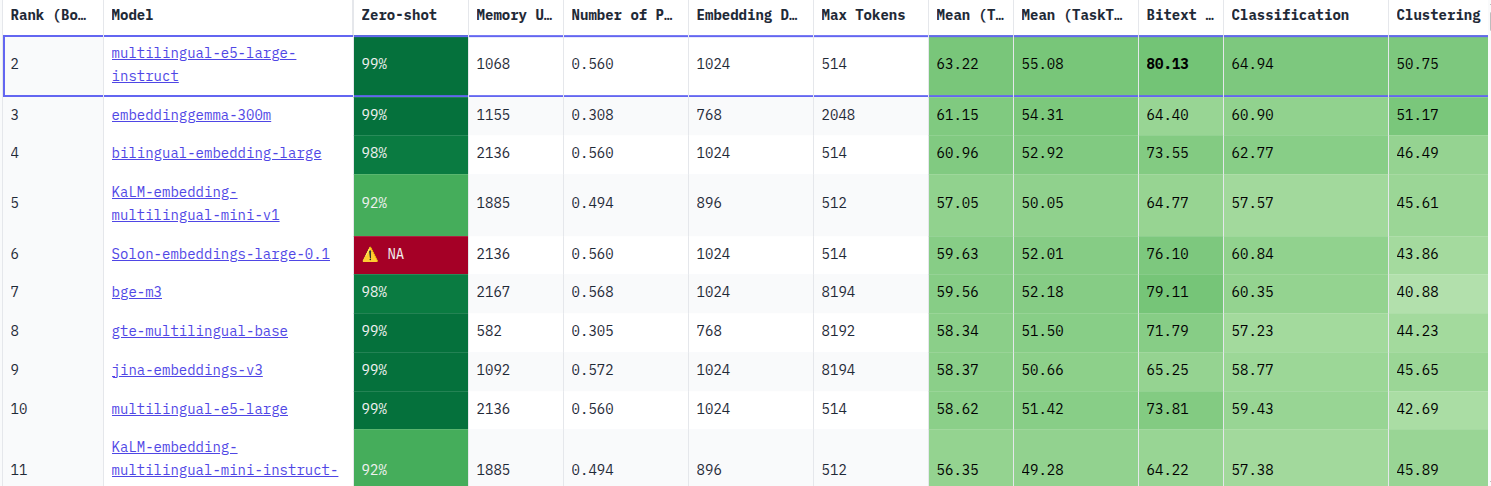
\includegraphics[width=\textwidth, keepaspectratio]{figures/mteb_multilingual_comparison.png}
    \end{figure}
    
    \textbf{\color{MainNavy}Choix : Multilingual-E5-large-instruct}
    \begin{itemize}
        \item 560M paramètres, entraîné sur 100+ langues
        \item Surpasse les autres modèles <1B params sur le benchmark multilingue MTEB
        \item Capacité de suivi d'instructions pour une meilleure compréhension des requêtes
    \end{itemize}
\end{frame}

\begin{frame}{Phase de Requête en Ligne}
    \begin{figure}
        \centering
        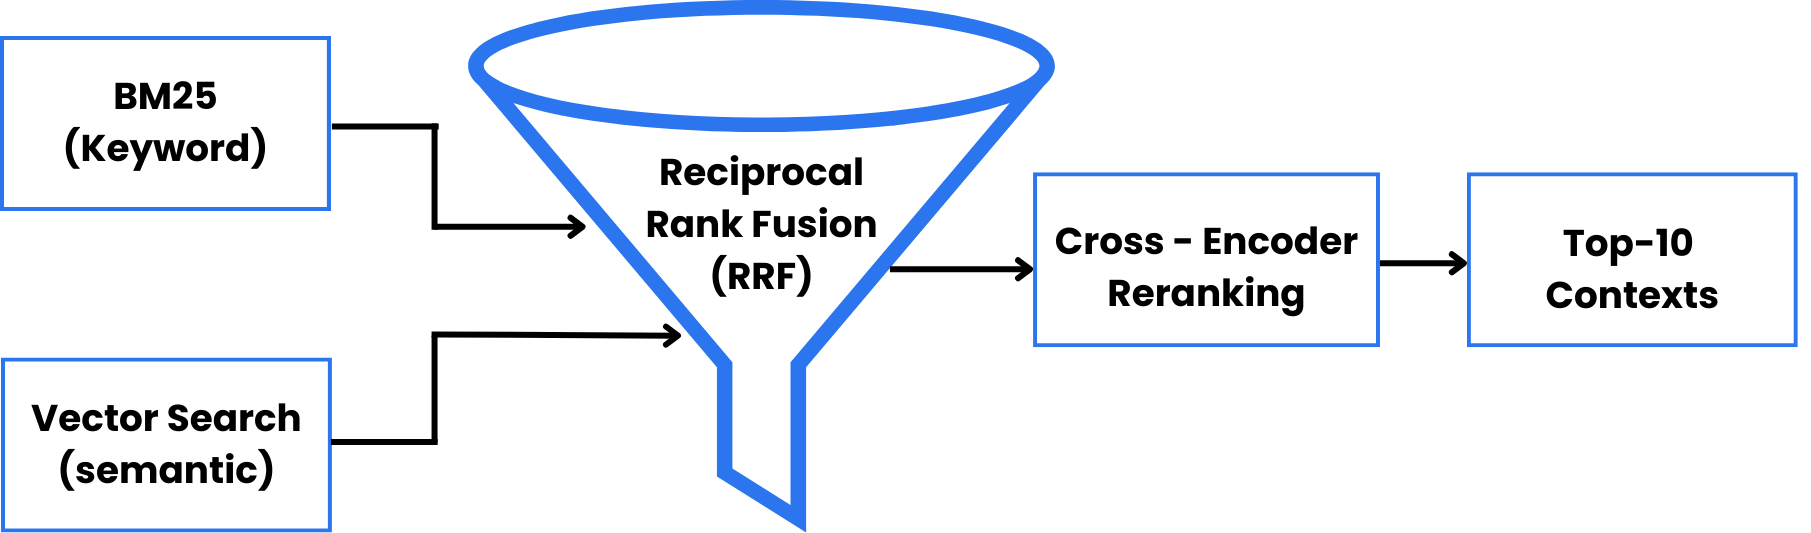
\includegraphics[width=0.65\textwidth]{figures/querying2.png}
    \end{figure}

    \footnotesize
    \textbf{Combinaison de Deux Approches :}
    \begin{itemize}
        \item \textbf{BM25 (Mots-clés) :} Correspondance exacte de termes pour les codes, noms
        \item \textbf{Recherche Vectorielle (Sémantique) :} Compréhension contextuelle
        \item \textbf{Fusion de Rang Réciproque :} Fusionner les résultats intelligemment
    \end{itemize}

    \textbf{Processus de Reclassement :}
    \begin{enumerate}
        \item La recherche hybride récupère les documents candidats
        \item Le cross-encoder calcule les scores de pertinence pour chaque paire requête-document
        \item Les top-k documents les plus pertinents sont envoyés au LLM pour génération
    \end{enumerate}
    
    \textbf{Avantage :} Traite le problème "perdu au milieu" en assurant que le contexte le plus pertinent est bien classé
\end{frame}

\begin{frame}{Configuration de l'Évaluation Expérimentale}
    \footnotesize 
    \begin{block}{Jeux de Données de Test}
        \begin{itemize}
            \item \textbf{Ensemble de Test GPM :} 25 questions complexes sur les rapports financiers de GPM
            \item \textbf{Ensemble de Test CCAM :} 10 scénarios de consultation clinique (fournis par Dr. Besnier)
        \end{itemize}
    \end{block}

    \begin{block}{Évaluation LLM-as-a-Judge utilisant les Métriques RAGAS}
        \begin{itemize}
            \item Deux modèles juges : \texttt{gemma-3-12b-it}, \texttt{mistral-small-24b-instruct-2501}
            \item Toutes les métriques sur échelle continue [0, 1], moyennées sur les deux juges
        \end{itemize}
    \end{block}

    \begin{table}
        \centering
        \small
        \begin{tabular}{lp{8cm}}
            \toprule
            \textbf{Métrique} & \textbf{Définition} \\
            \midrule
            Exactitude de Réponse & Similarité sémantique : générée vs. vérité terrain \\
            Pertinence de Réponse & Dans quelle mesure la réponse traite la requête \\
            Fidélité & Réponse ancrée dans le contexte récupéré \\
            Précision du Contexte & Chunks pertinents bien classés \\
            Taux de Réussite de Code@k & Code correct dans les top-k résultats (CCAM uniquement) \\
            \bottomrule
        \end{tabular}
    \end{table}
\end{frame}

\begin{frame}{Résultats : Amélioration Supérieure de la Précision}
    \begin{table}[H]
        \centering
        \caption{Résultats sur l'Ensemble de Test GPM (25 questions)}
        \small
        \begin{tabular}{|l|c|c|c|c|}
            \hline
            \textbf{Pipeline} & \textbf{Exact.} & \textbf{Pert.} & \textbf{Fidél.} & \textbf{Préc.} \\
            \hline
            RAG Simple & 0.648 & 0.788 & 0.732 & 0.654 \\
            \hline
            RAG Avancé & \textbf{0.976} & \textbf{0.972} & \textbf{0.940} & \textbf{0.960} \\
            \hline
            \textit{Amélioration} & \textit{+32.8\%} & \textit{+18.4\%} & \textit{+20.8\%} & \textit{+30.6\%} \\
            \hline
        \end{tabular}
    \end{table}

    \begin{table}[H]
        \centering
        \caption{Résultats sur l'Ensemble de Test CCAM (10 scénarios)}
        \small
        \begin{tabular}{|l|c|c|}
            \hline
            \textbf{Pipeline} & \textbf{Taux@5} & \textbf{Taux@20} \\
            \hline
            RAG Simple & 0.4 & 0.6 \\
            \hline
            RAG Avancé & \textbf{0.8} & \textbf{0.9} \\
            \hline
            \textit{Amélioration} & \textit{+40\%} & \textit{+30\%} \\
            \hline
        \end{tabular}
    \end{table}
\end{frame}

\begin{frame}{Résultats : Comparaison Visuelle}
    \begin{figure}
        \centering
        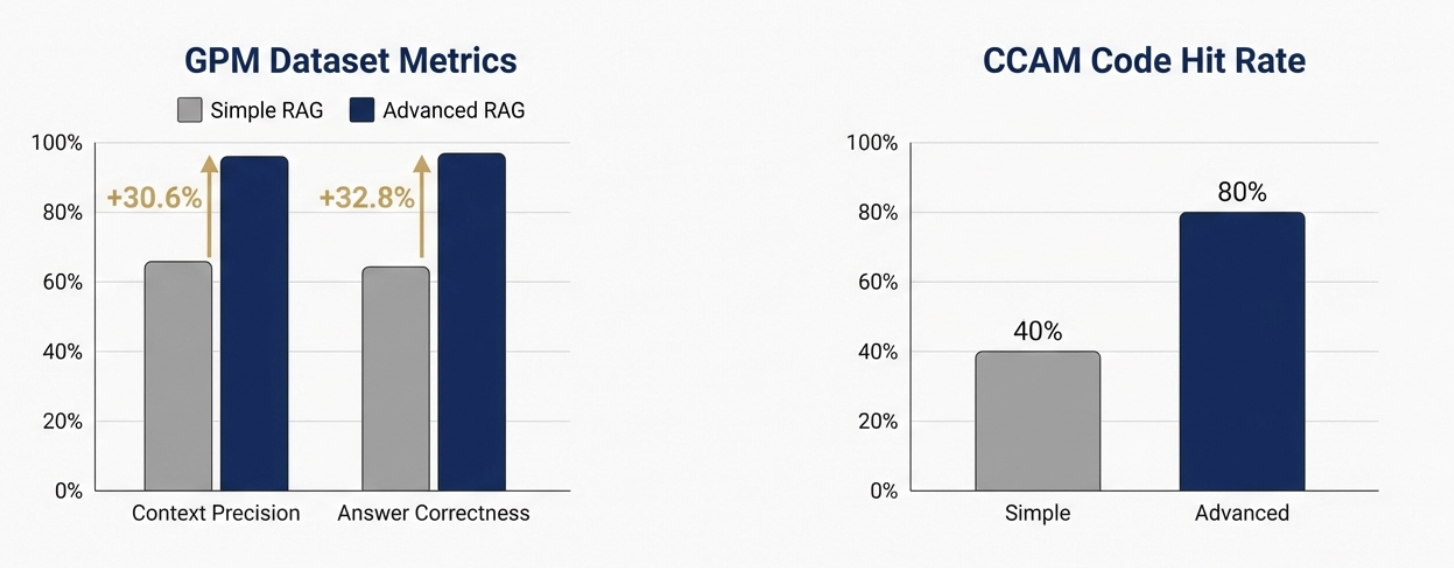
\includegraphics[width=0.8\textwidth]{figures/results_rag.png}
    \end{figure}
    \footnotesize
    \textbf{Observations Clés :}
    \begin{itemize}
        \item Le RAG avancé atteint des performances quasi-parfaites sur l'ensemble de données GPM
        \item Plus grandes améliorations en exactitude et précision du contexte
        \item Amélioration spectaculaire de la récupération exacte de code pour CCAM
        \item Gains cohérents sur toutes les métriques d'évaluation
    \end{itemize}
\end{frame}

\begin{frame}{Étude d'Ablation : Contribution de Chaque Composant}
    \begin{table}[H]
        \centering
        \caption{Améliorations incrémentales sur l'Ensemble de Test GPM}
        \small
        \begin{tabular}{|l|c|c|c|}
            \hline
            \textbf{Configuration} & \textbf{Précision} & \textbf{$\Delta$ vs Base} & \textbf{$\Delta$ Cumulatif} \\
            \hline
            Référence (RAG Simple) & 0.648 & --- & --- \\
            \hline
            + Analyse UnstructuredIO & 0.762 & +11.4\% & +11.4\% \\
            \hline
            + Résumé & 0.818 & +5.6\% & +17.0\% \\
            \hline
            + Embedding E5 Multilingue & 0.875 & +5.7\% & +22.7\% \\
            \hline
            + Recherche Hybride & 0.920 & +4.5\% & +27.2\% \\
            \hline
            + Reclassement & \textbf{0.976} & +5.6\% & \textbf{+32.8\%} \\
            \hline
        \end{tabular}
    \end{table}

    \textbf{Insights Clés :}
    \begin{itemize}
        \item La préservation de structure (UnstructuredIO) donne le plus grand gain unique (+11.4\%)
        \item Chaque composant contribue de manière significative à la performance finale
        \item L'effet cumulatif démontre la valeur de la conception holistique du pipeline
    \end{itemize}
\end{frame}

% ========== SECTION 3 : PROBLÈME 2 ==========
\section{Problème 2 : Adaptation Comportementale pour Petits Modèles}

% Slide de séparation de section
\begin{frame}[plain]
    \begin{center}
        \vfill
        {\Huge\color{MainNavy}\textbf{Problème 2}}
        \vspace{0.5cm}
        
        {\Large Adaptation Comportementale et Optimisation des Ressources pour Petits Modèles}
        \vspace{0.3cm}
        
        {\large Fine-tuning de Petits Modèles pour Tâches Spécialisées}
        \vfill
    \end{center}
\end{frame}

\begin{frame}{Problème 2 : Adaptation Comportementale pour Petits Modèles}
    \textbf{Contexte :} Construction d'un chatbot pour la lecture de Tarot (conseil psychologique)
    
    \vspace{0.3cm}
    \textbf{Approche Naïve :} Ingénierie de prompts avec de grands LLM (GPT-4, Claude-3) via API
    
    \vspace{0.3cm}
    \textbf{Pourquoi l'Ingénierie de Prompts Seule Est Insuffisante :}
    \begin{itemize}
        \item \textbf{Dilution de l'attention :} Contexte important perdu dans les longs prompts
        \item \textbf{Inconsistance :} Dérive hors caractère dans les conversations étendues
        \item \textbf{Coût :} Grands modèles coûteux pour le déploiement continu
    \end{itemize}

    \vspace{0.3cm}
    \begin{table}[H]
        \centering
        \caption{Comparaison des coûts opérationnels. *10K conversations × 3K tokens chacune. **Coût GPU amorti.}
        \small
        \begin{tabular}{|l|c|c|}
            \hline
            \textbf{Option} & \textbf{Coût/1K tokens} & \textbf{Coût/mois*} \\
            \hline
            API GPT-4-turbo & \$0.01--0.03 & \$300--900 \\
            API Claude 3 Sonnet & \$0.003--0.015 & \$90--450 \\
            Qwen-1.5B Fine-tuné & \$0.0005** & \$10--50 \\
            Qwen-0.5B Fine-tuné (Edge) & \$0 & \$0  \\
            \hline
        \end{tabular}
    \end{table}
\end{frame}

\begin{frame}{Exigences Spécifiques pour une Tâche de Lecture de Tarot}
     \begin{columns}[c]
        \begin{column}{0.32\textwidth}
            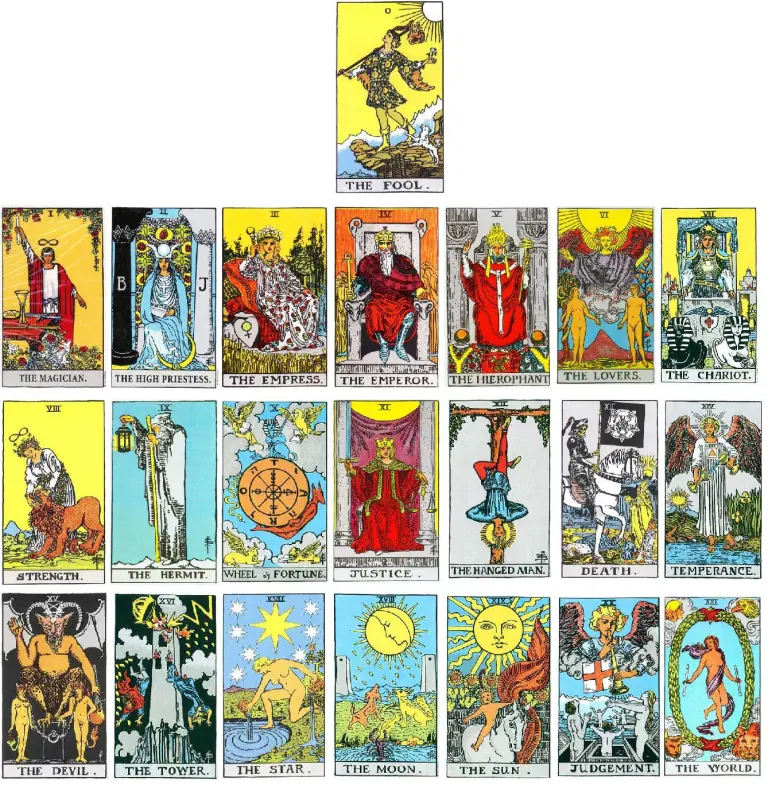
\includegraphics[width=\textwidth, keepaspectratio]{figures/tarot_cards.png}
            
            \small\textbf{Connaissances :} Significations des cartes et tirages
        \end{column}
        
        \begin{column}{0.32\textwidth}
            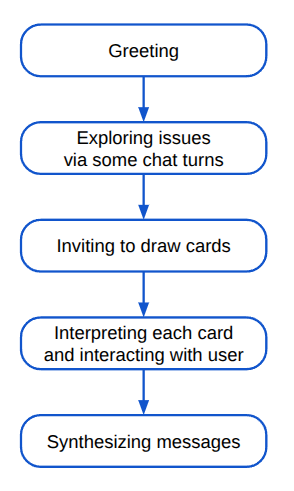
\includegraphics[width=0.9\textwidth, keepaspectratio]{figures/tarot_workflow.png}
            
            \small\textbf{Workflow :} Structure de conversation stricte
        \end{column}
        
        \begin{column}{0.32\textwidth}
            \textbf{Traits Comportementaux :}
            \begin{itemize}
                \small
                \item Ton empathique
                \item Interaction ouverte
                \item Éviter les prédictions directes
            \end{itemize}
        \end{column}
    \end{columns}
    
    \vspace{0.4cm}
    \textbf{\color{MainNavy}Défi :} Comment encoder toutes ces exigences dans un modèle petit et efficace ?
\end{frame}

\begin{frame}{Exemple d'une Conversation de Tarot}
    \begin{figure}
        \centering
        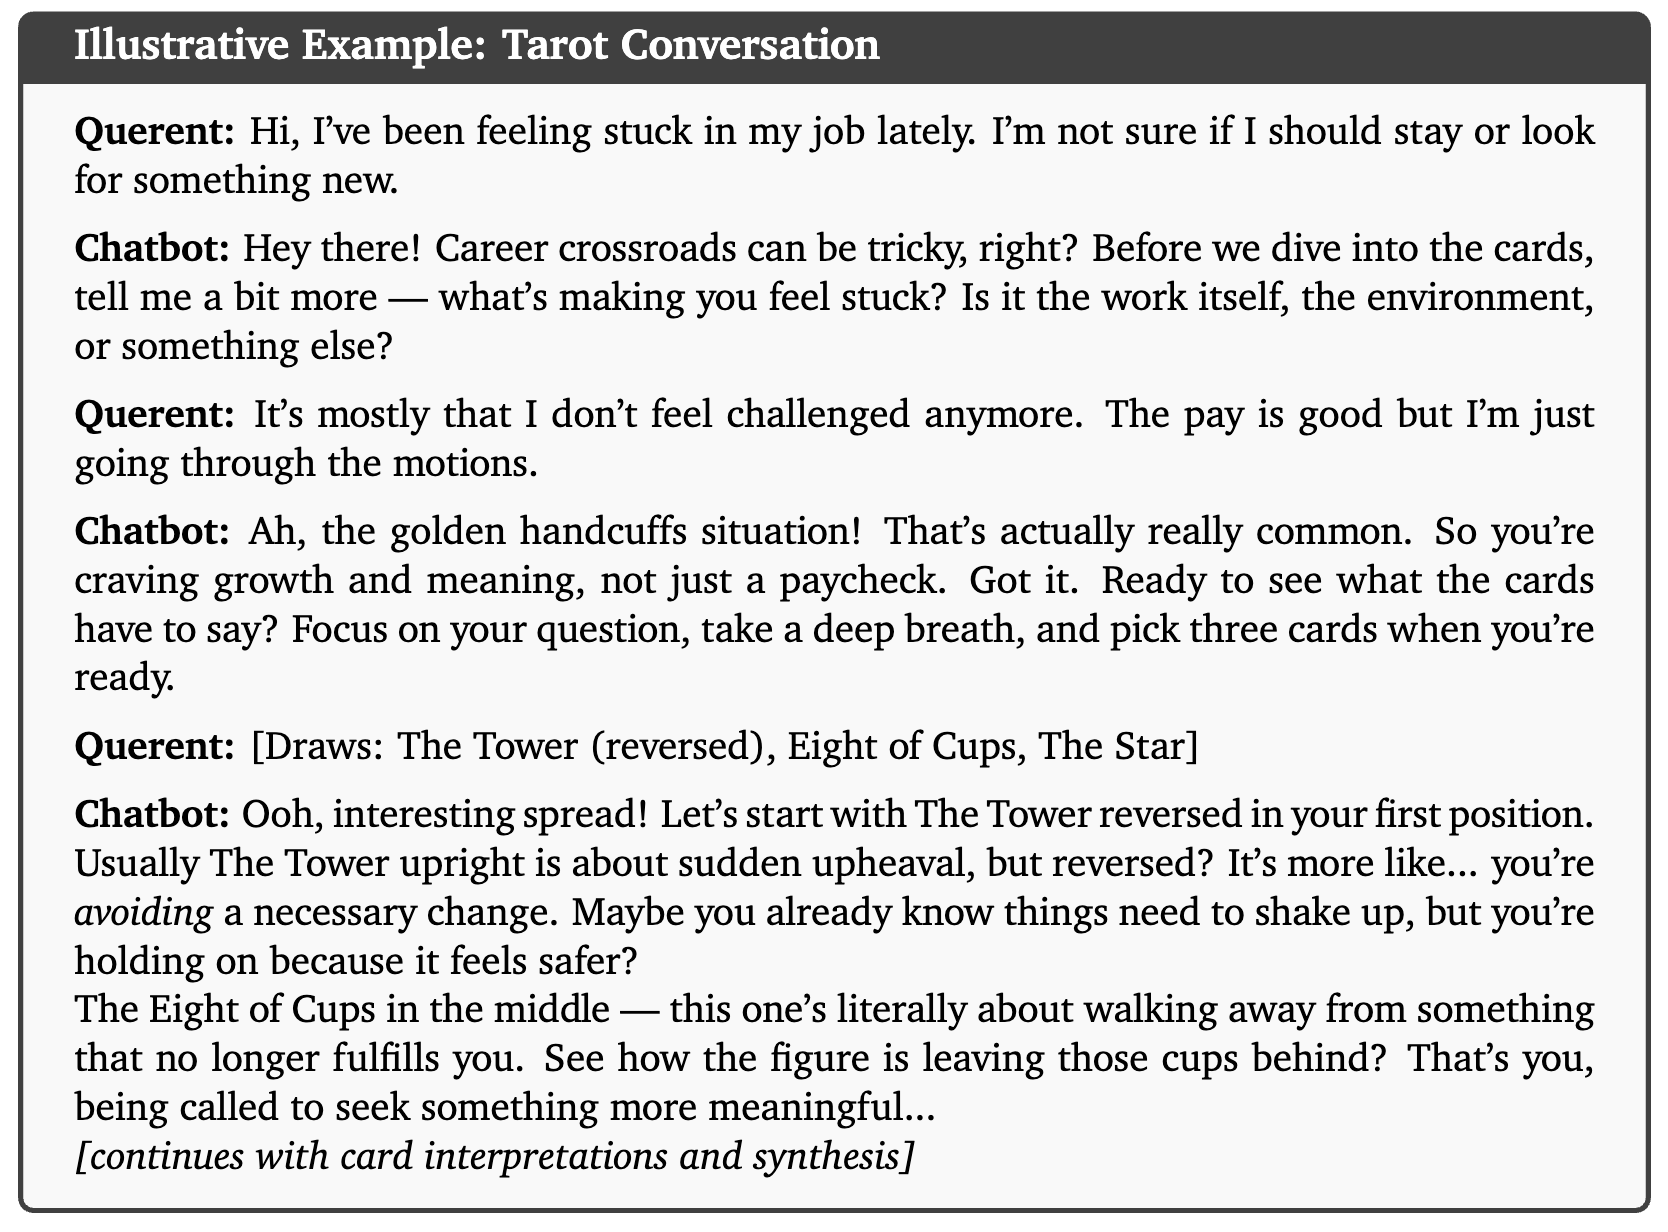
\includegraphics[height=0.85\textheight]{figures/tarot_conversation.png}
    \end{figure}
\end{frame}

\begin{frame}{Pipeline de Distillation : Génération de Données d'Entraînement Synthétiques}
    \begin{figure}
        \centering
        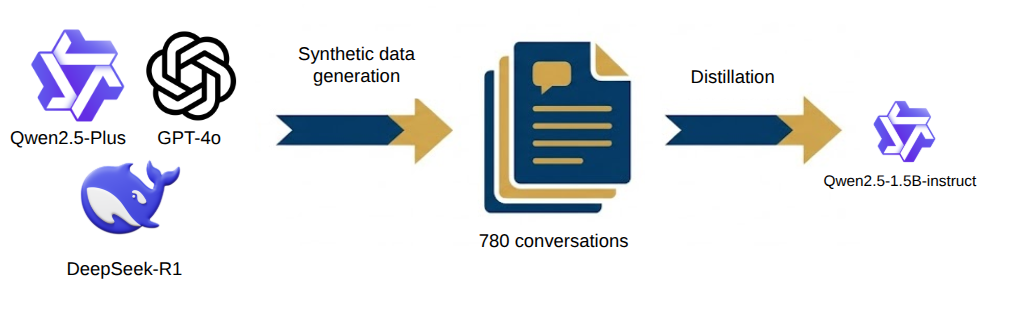
\includegraphics[width=\textwidth]{figures/distillation_pipeline.png}
    \end{figure}
    \footnotesize
    \textbf{Processus de Génération de Données :}
    \begin{itemize}
        \item Les LLM (Qwen2.5-Plus, GPT-4o, DeepSeek-R1) génèrent 780 conversations
        \item Chaque conversation inclut :
        \begin{itemize}
            \item Sujets et questions simulés des consultants
            \item Longueur de conversation spécifiée
            \item Traits de personnalité du consultant
            \item Combinaisons de cartes aléatoires avec leurs significations
        \end{itemize}
    \end{itemize}
\end{frame}

\begin{frame}{Sélection du Modèle : Pourquoi Qwen2.5-1.5B-Instruct ?}
    \begin{table}[H]
            \centering
            \caption{Performance sur benchmarks standards (Source : Rapport Technique Qwen2.5, 2024)}
            \small
            \begin{tabular}{lcccc}
                \toprule
                \textbf{Modèle} & \textbf{Params} & \textbf{MMLU} & \textbf{GSM8K} & \textbf{MATH} \\
                 & & (Connaiss.) & (Raisonn.) & (Logique Dure) \\
                \midrule
                Llama-3.2-1B-Instruct & 1.23B & 49.3 & 44.4 & 30.6 \\
                Gemma-2-2.6B-Base & 2.6B & 52.2 & 30.3 & 25.3 \\
                \textbf{Qwen2.5-0.5B-Instruct} & \textbf{0.49B} & 47.5 & \textbf{49.6} & \textbf{34.4} \\
                \textbf{Qwen2.5-1.5B-Instruct} & \textbf{1.54B} & \textbf{60.9} & \textbf{73.2} & \textbf{55.2} \\
                \bottomrule
            \end{tabular}
        \end{table}

    \textbf{Raisons de la Sélection :}
    \begin{enumerate}
        \item Ratio performance/paramètres supérieur
        \item Forte capacité multilingue
        \item Excellente capacité de suivi d'instructions
        \item Inférence efficace sur matériel grand public
    \end{enumerate}
\end{frame}

\begin{frame}{Résultats du Fine-tuning : Évaluation Complète}
    \begin{table}[H]
        \centering
        \caption{Résultats LLM-as-a-Judge (FT = Fine-tuné)}
        \tiny
        \begin{tabular}{|l|c|c|c|c|c|c|}
            \hline
            \textbf{Modèle} & \textbf{Style} & \textbf{Connaiss.} & \textbf{Empathie} & \textbf{Workflow} & \textbf{Cohér.} & \textbf{Moy} \\
            \hline
            \multicolumn{7}{|c|}{\textit{Juge : Gemma-3-12B-Instruct}} \\
            \hline
            Qwen-0.5B (base) & 0.42 & 0.65 & 0.48 & 0.35 & 0.72 & 0.52 \\
            Qwen-0.5B (FT) & 0.78 & 0.72 & 0.81 & 0.85 & 0.80 & 0.79 \\
            Qwen-1.5B (base) & 0.55 & 0.71 & 0.58 & 0.42 & 0.78 & 0.61 \\
            \rowcolor{gray!20}
            Qwen-1.5B (FT) & \textbf{0.88} & 0.85 & \textbf{0.89} & \textbf{0.92} & 0.88 & \textbf{0.88} \\
            GPT-4 (prompt) & 0.82 & 0.90 & 0.85 & 0.75 & 0.92 & 0.85 \\
            \hline
            \multicolumn{7}{|c|}{\textit{Juge : Mistral-Small-24B-Instruct}} \\
            \hline
            Qwen-1.5B (base) & 0.52 & 0.68 & 0.55 & 0.40 & 0.75 & 0.58 \\
            \rowcolor{gray!20}
            Qwen-1.5B (FT) & \textbf{0.85} & 0.82 & \textbf{0.86} & \textbf{0.90} & 0.86 & \textbf{0.86} \\
            GPT-4o (prompt) & 0.80 & \textbf{0.88} & 0.82 & 0.72 & \textbf{0.90} & 0.82 \\
            \hline
        \end{tabular}
    \end{table}
    
    \textbf{Résultats Clés :}
    \begin{itemize}
        \item Le fine-tuning améliore considérablement les métriques comportementales, en particulier la conformité au workflow (+50\% : 0.42 → 0.92)
        \item Qwen-1.5B fine-tuné surpasse GPT-4 avec prompts sur le style, l'empathie et le workflow
        \item Réduction de coût de 100x avec performance comparable ou meilleure
    \end{itemize}
\end{frame}

\begin{frame}{Application Démo utilisant Gradio}
    \begin{figure}
        \centering
        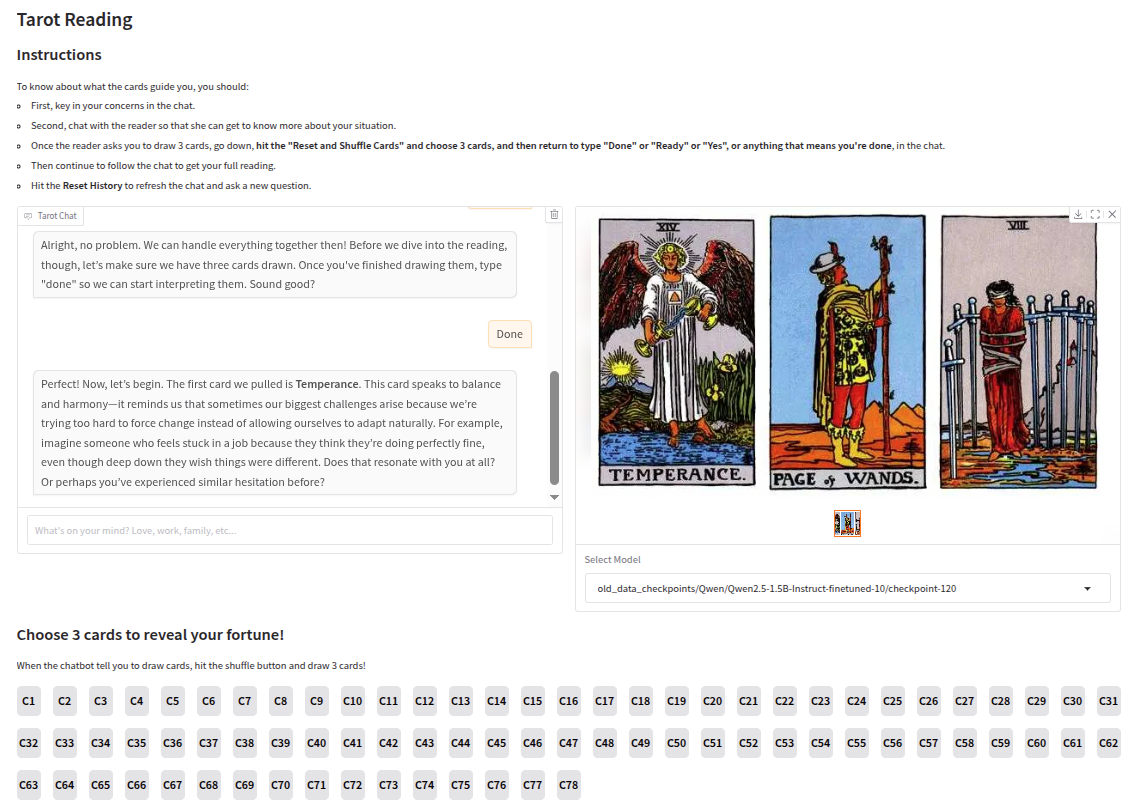
\includegraphics[width=0.5\textwidth]{figures/demo_tarot_application.png}
    \end{figure}
    \footnotesize
    \textbf{Fonctionnalités :}
    \begin{itemize}
        \item Sélection de cartes en temps réel avec retour visuel
        \item Conversation multi-tours avec préservation du contexte
        \item Changement de modèle pour comparaison
    \end{itemize}
\end{frame}

% ========== SECTION 4 : CONCLUSION ==========
\section{Conclusion}

\begin{frame}[plain]
    \begin{center}
        \vfill
        {\Huge\color{MainNavy}\textbf{Conclusion et Perspectives}}
        \vspace{0.5cm}
            
        \vfill
    \end{center}
\end{frame}

\begin{frame}{Contributions Clés}
    \textbf{\color{MainNavy}Problème 1 : Pipeline RAG Avancé}
    \begin{itemize}
        \item Développé un système RAG multimodal préservant la structure
        \item Atteint \textbf{32.8\% d'amélioration} de l'exactitude des réponses sur les documents financiers
        \item Atteint \textbf{40\% d'amélioration} du taux de réussite de code pour les documents médicaux
        \item Démontré la valeur de chaque composant du pipeline par étude d'ablation
    \end{itemize}
    
    \vspace{0.3cm}
    \textbf{\color{MainNavy}Problème 2 : Adaptation Comportementale par Fine-tuning}
    \begin{itemize}
        \item Conçu un pipeline de distillation efficace pour petits modèles
        \item Qwen-1.5B fine-tuné surpasse GPT-4 avec prompts sur les métriques comportementales
        \item Atteint \textbf{80-90\% de réduction de coût} tout en maintenant une performance comparable
        \item Démontré la faisabilité d'agents conversationnels spécialisés sur matériel grand public
    \end{itemize}
    
    \vspace{0.3cm}
    \textbf{\color{MainNavy}Impact Global}
    \begin{itemize}
        \item Fourni des solutions pratiques aux lacunes de connaissances et de comportement
        \item Permis le déploiement dans des environnements à enjeux élevés et ressources limitées
    \end{itemize}
\end{frame}

\begin{frame}{Directions Futures}
    \textbf{\color{MainNavy}Améliorations à Court Terme :}
    \begin{itemize}
        \item Évaluation étendue sur des ensembles de données spécifiques au domaine supplémentaires
        \item Optimisation pour le déploiement en périphérie (quantification, élagage)
    \end{itemize}
    
    \vspace{0.3cm}
    \textbf{\color{MainNavy}Directions de Recherche à Long Terme :}
    \begin{itemize}
        \item \textbf{RLHF :} Apprentissage par renforcement à partir de retours humains pour mieux aligner les sorties du modèle avec les attentes des utilisateurs
        \item \textbf{Génération Multimodale :} Extension au-delà du texte pour soutenir les explications visuelles (par ex. génération de graphiques dans les rapports financiers)
        \item \textbf{Support Multilingue :} Extension pour soutenir des bases d'utilisateurs mondiales dans plusieurs langues
    \end{itemize}
\end{frame}

\begin{frame}[plain]
    \begin{center}
        \vfill
        {\Huge\color{MainNavy}\textbf{Merci}}
        \vspace{0.5cm}
        
        {\Large Session de Questions-Réponses}
        \vspace{1cm}
        
        \textbf{Contact :}
        
        Minh Duy Nguyen
        
        \texttt{mnguye@insa-toulouse.fr}
        \vfill
    \end{center}
\end{frame}

\end{document}